% !TEX program = xelatex
\documentclass[11pt, aspectratio=169]{beamer}
\usetheme{metropolis}
\useoutertheme{metropolis}
\useinnertheme{metropolis}
\usecolortheme{metropolis}
\usefonttheme{professionalfonts} % [Beamer 설정] Beamer가 폰트를 건드리지 못하게 함 (필수)

\usepackage{kotex}
\usepackage{tikz} 
\usepackage{graphicx, caption, hyperref, fontawesome5}
% [추가] subfigure 환경을 사용하기 위해 필수입니다!
\usepackage{subcaption}

% [수식 및 폰트 핵심 설정]
\usepackage{amsmath}
\usepackage[math-style=ISO, bold-style=ISO]{unicode-math} % unicode-math 로드

% 1. Beamer가 폰트를 제멋대로 바꾸지 못하게 막음 (필수!)
\usefonttheme{professionalfonts}

% 2. 본문 폰트 설정 (Pretendard)
% AutoFakeSlant: 이탤릭체가 없는 Pretendard를 위해 강제로 20% 기울임
\setmainfont[Ligatures=TeX, BoldFont={* Bold}, AutoFakeSlant=0.2]{Pretendard}
\setsansfont[Ligatures=TeX, BoldFont={* Bold}, AutoFakeSlant=0.2]{Pretendard}
\setmainhangulfont[BoldFont={* Bold}]{Pretendard}
\setsanshangulfont[BoldFont={* Bold}]{Pretendard}

% 3. 수식 폰트 설정 (Fira Math + Pretendard 조합)
% (A) 기본 수식 기호는 Fira Math (Sans-serif Math Font) 사용
\setmathfont{Fira Math}

% (B) 수식 내의 문자(x, y, log, sin 등)는 Pretendard로 덮어씌움 (통일감)
\setmathfont[range={up, bfup}, Scale=MatchLowercase]{Pretendard}
\setmathfont[range={it, bfit}, Scale=MatchLowercase, FakeSlant=0.2]{Pretendard}

% 4. 메타데이터
\title{Communication Theory - 2026}
\subtitle{CDMA 시스템과 Viterbi 복호화}
\date{\today}
\author{
    이 경 근 \\
    {\tiny
        \raisebox{0.1ex}{\scalebox{0.85}{\faEnvelope}} \href{mailto:infosec@knu.ac.kr}{infosec@knu.ac.kr} \quad 
        {\scalebox{0.9}{\faLinkedin}} \scalebox{0.9}{\href{https://www.linkedin.com/in/Kenny-0633-Lee}{Kenny-0633-Lee}}
    }
}
\institute{EE / KNU}
\graphicspath{ {./} {../../assets/} {../assets/} }


%%%%%%%%%%%%%%%%%%%%%%%%%%%%%%%%%%%%%%%%%%%%%
%%%%%%%%%%%%%%%%%%%%%%%%%%%%%%%%%%%%%%%%%%%%%

\begin{document}

% Title Page
\begin{frame}[plain]
    \titlepage
\end{frame}

% \begin{frame}
%     \[
%         \int_0^{\pi} \sin x \, \mathrm{d}x = 2
%     \]

% \end{frame}

% --- Introduction ---
\begin{frame}{Introduction}
    \centering
    Python과 LaTeX의 완벽한 분리(Decoupling)를 통한\\
    \textbf{안정적인 강의 자료 시스템}입니다.
\end{frame}

% --- 강의 범위 및 시각화 계획 (Lathi Ch 1-7) ---
\begin{frame}{강의 범위 및 시각화 계획 (Lathi Ch 1-7)}
    \begin{itemize}
        \item \textbf{Ch 1-3:} 신호와 시스템 (Time/Freq Plot)
        \item \textbf{Ch 4-5:} 아날로그 변조 (AM/FM Waveform)
        \item \textbf{Ch 6-7:} 디지털 통신 (Sampling, Constellation)
    \end{itemize}
\end{frame}

% ... (이전 "강의 범위 및 시각화 계획" 프레임 끝) ...

% --- [NEW] Ch 01. Shannon Theory ---
\begin{frame}{Chapter 01. Why Bandwidth is Revenue}
    \begin{columns}
        % [Left] Python Generated Visual
        \begin{column}{0.6\textwidth}
            \centering
            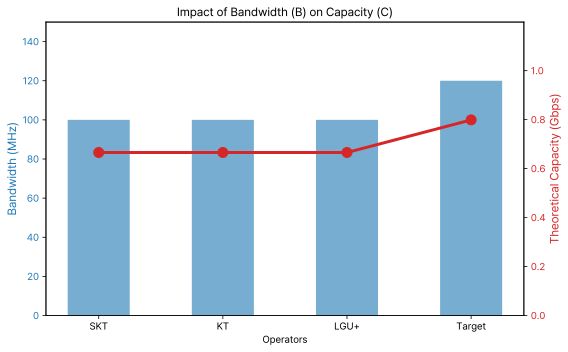
\includegraphics[width=\textwidth]{fig_ch01_shannon}
        \end{column}
        
        % [Right] Mathematical Proof
        \begin{column}{0.4\textwidth}
            \begin{block}{Shannon-Hartley Theorem}
                \centering
                $C = \mathbf{B} \log_2 \left( 1 + \frac{S}{N} \right)$
            \end{block}
            
            \vspace{0.3cm}
            \textbf{Key Insight:}
            \begin{itemize}
                \item \textbf{Bandwidth ($\mathbf{B}$):} \\
                Capacity와 \textcolor{red}{선형(Linear)} 비례 \\
                $\rightarrow$ \textit{"돈으로 대역폭을 사는 이유"}
                
                \item \textbf{Power ($S$):} \\
                Capacity와 \textcolor{blue}{로그(Log)} 비례 \\
                $\rightarrow$ \textit{"효율 체감의 법칙"}
            \end{itemize}
        \end{column}
    \end{columns}
\end{frame}

% --- 5G Spectrum ---
\begin{frame}{Practical Application: 5G Spectrum in Korea}
    \centering
    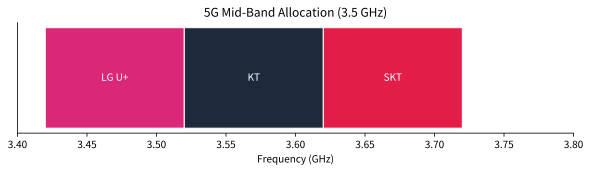
\includegraphics[width=0.9\textwidth]{fig_ch3_5g_spectrum}
    
    \vspace{0.5cm}
    \begin{block}{Shannon-Hartley Theorem in Practice}
        $C = \mathbf{B} \log_2(1 + SNR)$
        \begin{itemize}
            \item \textbf{mmWave (28GHz):} $B = 800\text{MHz}$ $\rightarrow$ Ultra-high Capacity
            \item \textbf{Sub-6 (3.5GHz):} $B = 100\text{MHz}$ $\rightarrow$ National Coverage
        \end{itemize}
    \end{block}
    \small \textit{Observation: 광대역 연속 블록 확보가 스펙트럼 효율의 핵심입니다.}
\end{frame}

% --- Chapter 2 Preview ---
\begin{frame}{Chapter 2 Preview: The Fourier Series}
    \framesubtitle{All signals are sums of sinusoids}
    
    % 그림 3개를 가로로 나란히 배치
    \begin{figure}
        \centering
        \begin{subfigure}{0.32\textwidth}
            \includegraphics[width=\linewidth]{fourier_step_1}
            \caption{N=1 (Fundamental)}
        \end{subfigure}
        \hfill
        \begin{subfigure}{0.32\textwidth}
            \includegraphics[width=\linewidth]{fourier_step_5}
            \caption{N=5 (Adding Harmonics)}
        \end{subfigure}
        \hfill
        \begin{subfigure}{0.32\textwidth}
            \includegraphics[width=\linewidth]{fourier_step_29}
            \caption{N=29 (Square Wave)}
        \end{subfigure}
        
        \caption{Gibbs Phenomenon visualized using Python}
    \end{figure}
    
    \begin{itemize}
        \item We will learn how to decompose any signal into simple sine waves.
    \end{itemize}
\end{frame}

% --- Chapter 2 Preview ---
\begin{frame}{Chapter 2 Preview: The Fourier Series}
    \framesubtitle{All signals are sums of sinusoids}
    
    % 1. figure 환경을 먼저 엽니다.
    \begin{figure}
        \centering
        
        % 2. 정지 이미지들 (Filmstrip)
        \begin{subfigure}{0.32\textwidth}
            \includegraphics[width=\linewidth]{fourier_step_1}
            \caption{N=1}
        \end{subfigure}
        \hfill
        \begin{subfigure}{0.32\textwidth}
            \includegraphics[width=\linewidth]{fourier_step_5}
            \caption{N=5}
        \end{subfigure}
        \hfill
        \begin{subfigure}{0.32\textwidth}
            \includegraphics[width=\linewidth]{fourier_step_29}
            \caption{Square Wave}
        \end{subfigure}
        
        \vspace{0.2cm}
        
        % 3. [핵심] 링크는 캡션 텍스트에만 겁니다.
        % (run: 뒤의 경로는 실제 파일 위치에 맞춰야 합니다)
        \caption{
            \href{run:../../assets/anim_01_square_wave_synthesis.gif}
            {\textcolor{blue}{\faPlayCircle \ Click here to play Animation}}
        }
    \end{figure}
    
    \begin{itemize}
        \item We will learn how to decompose any signal into simple sine waves.
    \end{itemize}
\end{frame}

% --- Ch 3. AM Frequency Shifting ---
\begin{frame}{Chapter 3. Amplitude Modulation (AM)}
    \framesubtitle{The Modulation Theorem: Frequency Shifting}
    
    \centering
    % 가로 너비를 화면의 90%로 설정하여 시원하게 보여줍니다.
    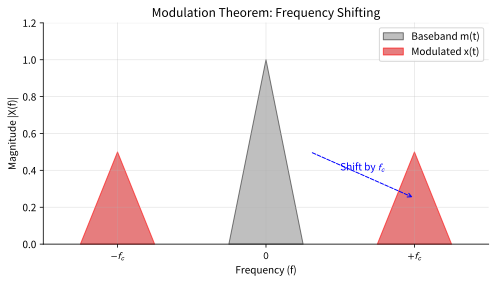
\includegraphics[width=0.9\textwidth]{fig_03_am_shift}
    
    \vspace{0.3cm}
    
    \begin{block}{Frequency Shifting Property}
        Time Domain에서 $\cos(2\pi f_c t)$를 곱하면,\\
        Frequency Domain에서는 스펙트럼이 $\pm f_c$로 \textbf{이사(Shift)} 갑니다.
        \[
            x(t) = m(t) \cos(2\pi f_c t) \iff X(f) = \frac{1}{2} [M(f-f_c) + M(f+f_c)]
        \]
    \end{block}
\end{frame}

% --- Ch 4. AM 예제 ---
\begin{frame}{Chapter 4. Amplitude Modulation}
    \begin{columns}
        \begin{column}{0.5\textwidth}
            \textbf{Time Domain}
            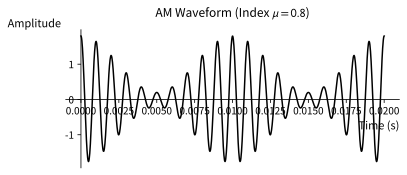
\includegraphics[width=\textwidth]{fig_ch4_am_time}
        \end{column}
        \begin{column}{0.5\textwidth}
            \textbf{Frequency Domain}
            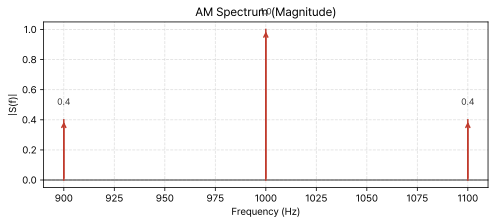
\includegraphics[width=\textwidth]{fig_ch4_am_spec}
        \end{column}
    \end{columns}
    \vspace{0.2cm}
    \centering
    \small AM 신호는 시간 영역의 포락선(Envelope)과 주파수 영역의 측파대(Sidebands)로 해석됩니다.
\end{frame}

% --- Ch 4. FM Accordion Effect ---
\begin{frame}{Chapter 4. Frequency Modulation (FM)}
    \framesubtitle{Visualizing Instantaneous Frequency}

    \begin{columns}
        % [Left Column] 그림 영역
        \begin{column}{0.6\textwidth}
            \centering
            % 높이를 화면의 80%로 맞춰서 위아래가 잘리지 않게 합니다.
            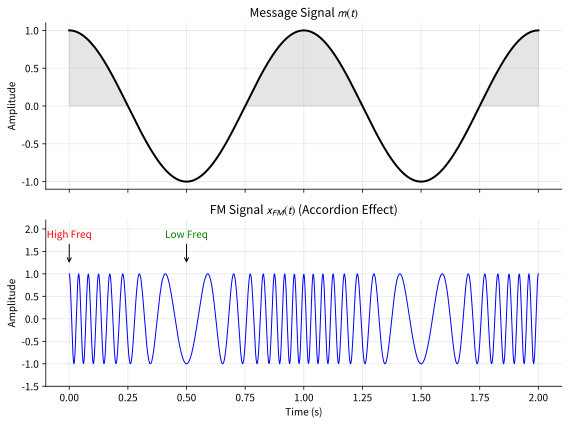
\includegraphics[height=0.8\textheight]{fig_04_fm_accordion}
        \end{column}
        
        % [Right Column] 설명 영역
        \begin{column}{0.4\textwidth}
            \textbf{The "Accordion" Effect}
            \vspace{0.2cm}
            \begin{itemize}
                \item \textbf{High Amplitude:} \\
                $\rightarrow$ 주파수가 높아짐 \\
                (파형이 촘촘해짐, Compressed)
                
                \vspace{0.3cm} % 항목 간 간격
                
                \item \textbf{Low Amplitude:} \\
                $\rightarrow$ 주파수가 낮아짐 \\
                (파형이 느슨해짐, Relaxed)
            \end{itemize}
            
            \vspace{0.5cm}
            \small
            \textit{Insight: 진폭(Amplitude)은 일정하므로 잡음(Noise)에 강합니다.}
        \end{column}
    \end{columns}
\end{frame}

% --- Ch 7. Digital 예제 ---
\begin{frame}{Chapter 7. Digital Modulation (QPSK)}
    \begin{columns}
        \begin{column}{0.6\textwidth}
            \centering
            % 정사각형 비율 유지를 위해 height 지정
            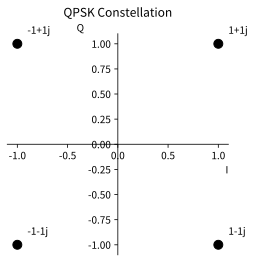
\includegraphics[height=0.6\textheight]{fig_ch7_qpsk}
        \end{column}
        \begin{column}{0.4\textwidth}
            \textbf{QPSK 특징:}
            \begin{itemize}
                \item 2 bits per symbol
                \item 4개의 위상 상태
                \item 대역폭 효율성 증대
            \end{itemize}
        \end{column}
    \end{columns}
\end{frame}


% --- Closing ---
\begin{frame}{강의 Recap.}
    \centering
    \begin{itemize}
        \item Python을 통한 신호 생성 및 시각화
        \item LaTeX Beamer로 안정적인 프레젠테이션 제작
        \item $C = \mathbf{B} \log_2 \left( 1 + \frac{S}{N} \right)$
        \item 통신 이론의 핵심 개념들을 시각적으로 이해
    \end{itemize}
\end{frame}

\end{document}